Dans le but d'effectuer une série de tests avec les capteur choisis, il a fallu simuler un environnement 
similaire aux conditions réelles. Le premier défi est de simuler de la neige en plein été. Etant donné 
que des canons à neige ou autres dispositifs équivalents n’étaient pas disponibles, de la fausse neige 
a dû être fabriquée. Cependant, simuler des chutes de neige implique des importantes salissures. Un 
banc de test a donc été mis en place pour effectuer ces tests de manière propre. Pour simuler la neige 
qui tombe, un canon à confettis a permis de le faire. Ces mesures ont grandement aidé à l’avancement 
du projet.\par 
Le deuxième grand défi est de compacter toute l'électronique dans un boitier pouvant résister aux 
intempéries. Une carte de développement, une carte d'extension, des batteries ainsi que d’autres composants 
doivent être à l’abri dans ce boitier. Pour assurer des mesures fiables et la survie de l’électronique, 
l’étanchéité du boitier est nécessaire. La simplicité du démontage est aussi recherchée, elle permettra 
aux personnes de gagner du temps lors du montage ou de la maintenance.

\section{Banc de test}

Durant l’étape de recherche, deux méthodes de mesure ont été retenues. Cependant, les possibilités pour 
attester de leur bon fonctionnement sont restreintes. Afin d’avoir un espace pour effectuer des tests 
volatiles sans impacter nos collègues, un banc d’essai a été mis en place. \\
Il est nécessaire que ce banc de test soit assez grand pour que trois personnes puissent effectuer des 
essais avec les capteurs choisis. Les nuages de confettis générés ne doivent en aucun cas gêner les 
autres personnes présentes dans la salle de classe. Une cage avec une base de 2m par 1.5m et 1.5m de 
haut a été développée. La figure \ref{fig:encombrement} montre les étapes de conception de ce banc 
de test.

\begin{figure}[H]
    \centering
    \includegraphics[width=0.3\textwidth]{Images/photos_PGA/P004_CageDeTest21.png}
    \includegraphics[width=0.3\textwidth]{Images/photos_PGA/P004_CageDeTest2.png}
    \includegraphics[width=0.3\textwidth]{Images/photos_PGA/IMG_0442.jpg}
    \caption{Encombrement de la structure de test}
    \label{fig:encombrement}
\end{figure}

Comme des essais doivent être réalisés dès les premières semaines du projet, la structure a dû être
rapidement construite. Une structure en bois a donc été retenue pour sa simplicité de montage. 
Les façades de la cage ont été réalisées avec des bâches de protections épaisses que nous avons aggrafé 
sur la structure. Les planches ont été assemblées à l’aide d’équerres en métal et de vis à bois.\\
Afin d’avoir une bonne rigidité, la structure aurait pu être triangulé avec des poutres en bois. 
Cependant, le banc de test étant exposé à quasiment aucune contrainte mécanique, la rigidité ajoutée par 
les bâches de protections est largement suffisante. Cette configuration nous a permis d’économiser du 
temps et de l’argent.

\subsection{Fausse neige (confettis)}

\subsubsection{Problématique}

Simuler de la neige en plein été représente un défi supplémentaire. La température ne jouant pas en notre 
faveur, la solution retenue est d’utiliser des confettis blancs. À la suite d’une commande impossible 
de confettis (rupture de stock), nous avons rapidement dû trouver une autre solution.

\subsubsection{Méthode}

La première idée envisagée consiste à regarder dans les bacs des perforatrices automatiques situées 
dans les imprimantes de l’école. Malheureusement ces derniers étaient vidés régulièrement. La quantité 
trouvée était plus qu’insuffisante.\\
La deuxième solution, celle qui a été retenue, est d’utiliser la déchiqueteuse du secrétariat. Cette 
démarche n’était pas des plus écologique, mais elle a permis de pouvoir créer les confettis rapidement. 
Un paquet de feuille blanche a été détruit pour fabriquer un carton plein de lamelle blanche s’apparentant 
à des confettis ou de la grosse neige. \\
Le remplissage du carton à la figure \ref{fig:confettis} a pris environ une heure. 

\begin{figure}[H]
    \centering
    \includegraphics[width=0.4\textwidth]{Images/photos_PGA/ConfBox.jpeg}
    \includegraphics[width=0.4\textwidth]{Images/photos_PGA/conf.jpeg}
    \caption{Aspect des confettis fabriqués}
    \label{fig:confettis}
\end{figure}

\subsection{Canon à confettis}

La meilleure solution pour simuler la chute des flocons est de projeter des confettis vers le haut 
de la manière la plus continue possible. Les premiers essais ont été effectués en les jetant manuellement 
devant les capteurs. Cependant, un débit constant était nécessaire afin de pouvoir effectuer des séries de
mesures et déterminer plus précisément les erreurs. 

\subsubsection{Principe de fonctionnement}

Des recherches concernant des solutions déja existantes ont été effectuées. Malheureusement, la plupart 
utilisent un principe d'à-coup d'air comprimé, un effet non désiré. Finalement, un canon avec un 
débit d'air plus faible a été retenu, fonctionnant par effet Venturi.
Le principe de base (inspiré des carburateurs) est, grâce à un débit d’air régulier dans 
notre cas, d’aspirer des confettis introduits dans un réservoir grâce à une baisse de pression à un 
endroit précis. La première version est constituée d’un tube principal avec une réduction de section, où
on retrouve un débit d'air constant. Les confettis sont stockés dans un réservoir au-dessus de la zone 
de dépression, d'où ils sont aspirés vers un petit coude, leur permettant de mieux couler dans le 
tube principal.\par 
Sur le schéma de la figure \ref{fig:venturi}, le principe du canon y est représenté. Le débit d’air constant 
(en noir) arrive au niveau du réservoir, la section diminuant, la pression diminue aussi. Ainsi, un phénomène 
d’aspiration se produit. De cette manière, un mélange d'air et de confettis est projeté.

\begin{figure}[H]
    \centering
    \includegraphics[width=0.5\textwidth]{Images/photos_PGA/venturi_v1b.PNG}
    \caption{Principe du canon à effet Venturi}
    \label{fig:venturi}
\end{figure}

Cette première version fut rapidement envoyée à l’atelier pour être imprimée afin d’effectuer 
les premiers tests et les éventuelles corrections du canon. La figure \ref{fig:3DPrintCanon} montre 
le tube principale imprimé en PETG grâce à l’imprimante 3D de l’école.

\begin{figure}[H]
    \centering
    \includegraphics[width=0.35\textwidth]{Images/photos_PGA/CanonBloc.jpg}
    \caption{Exemple d'impression 3D du canon}
    \label{fig:3DPrintCanon}
\end{figure}

\subsubsection{Turbine}

Un paramètre indispensable est d’avoir une source d’air continue avec un débit satisfaisant. La salle de classe étant 
équipée d’air comprimé, il suffit de l’utiliser pour avoir un débit d’air constant. Cependant, 
le bâtiment étant encore en travaux, les raccords d’air n’étaient pas sertis. Une autre solution doit 
être trouvée. Une turbine alimentée par un moteur à courant continue se trouve être la bonne 
solution. Premièrement, ce dispositif est relativement simple. En effet, pour régler la vitesse de rotations, il suffit 
de changer la tension aux bornes du moteur. Deuxièmement, la mécanique est facilement intégrable 
au canon. Cette solution permet de ne plus se soucier des problèmes de débit d’air. La figure \ref{fig:turbine}
montre la pièce d'adaptation entre la turbine et le tube principal.

\begin{figure}[H]
    \centering
    \includegraphics[width=0.25\textwidth]{Images/photos_PGA/adaptmotventi.PNG}
    \includegraphics[width=0.25\textwidth]{Images/photos_PGA/zoomTurbine.jpg}
    \caption{Turbine DC}
    \label{fig:turbine}
\end{figure}

\subsubsection{Problèmes rencontrés}

A la suite d'une série de tests, plusieurs éléments se sont révélés problématiques. Premièrement, les 
confettis confectionnés ont une tendance à s’enchevêtrer les uns dans les autres, et cela réduit 
considérablement leurs capacités à couler dans le réservoir. Ce dernier se retrouvait sans cesse 
bouché. Grace aux tests, le fait d’agrandir le passage des confettis permettrai d’avoir un meilleur 
écoulement et de limiter la formation de bouchons.

\subsubsection{Solution apportée}

En prenant en compte les problèmes survenu lors des premiers essais, une deuxième version a été modélisée, 
cette fois-ci avec un réservoir plus grand et un angle de remplissable plus faible. Le coude passe 
de 28mm de diamètre à 34 mm. Ce dernier est maintenant directement imprimé dans le tube principal afin 
d’éviter les angles trop saillants qui pourraient causer un blocage, comme le montre la figure \ref{fig:venturiv2}. 
Afin d’obtenir un coude plus large 
il a fallu augmenter le changement de section dans le tube principal. Nous aurions eu la possibilité de 
totalement refabriquer la pièce pour avoir une plus grande aspiration. Cependant, le fait de garder 
les dimensions de bases permettait de gagner du temps et d’éviter de relancer des impressions 3D inutilement.

\begin{figure}[H]
    \centering
    \includegraphics[width=0.4\textwidth]{Images/photos_PGA/venturi_v2.PNG}
    \caption{Deuxième version du canon}
    \label{fig:venturiv2}
\end{figure}

Lors des essais de la nouvelle version, le changement était notable. Le fait d’avoir augmenté le diamètre 
du coude et de l’avoir imprimé en une fois avec le tube principal a réduit fortement les angles saillants. 
Les lamelles de papiers continuaient à se coincer de temps en temps mais l’objectif d’avoir un débit 
constant pendant plus d'une minute a pu largement être atteint. Le canon était même capable s’il était 
placé réservoir vers le bas d’aspirer les confettis comme un aspirateur et de les rejeter comme de la 
neige. On peut voir sur la figure \ref{fig:canonupdate} le canon en action.

\begin{figure}[H]
    \centering
    \includegraphics[width=0.35\textwidth]{Images/photos_PGA/canonAction1.PNG}
    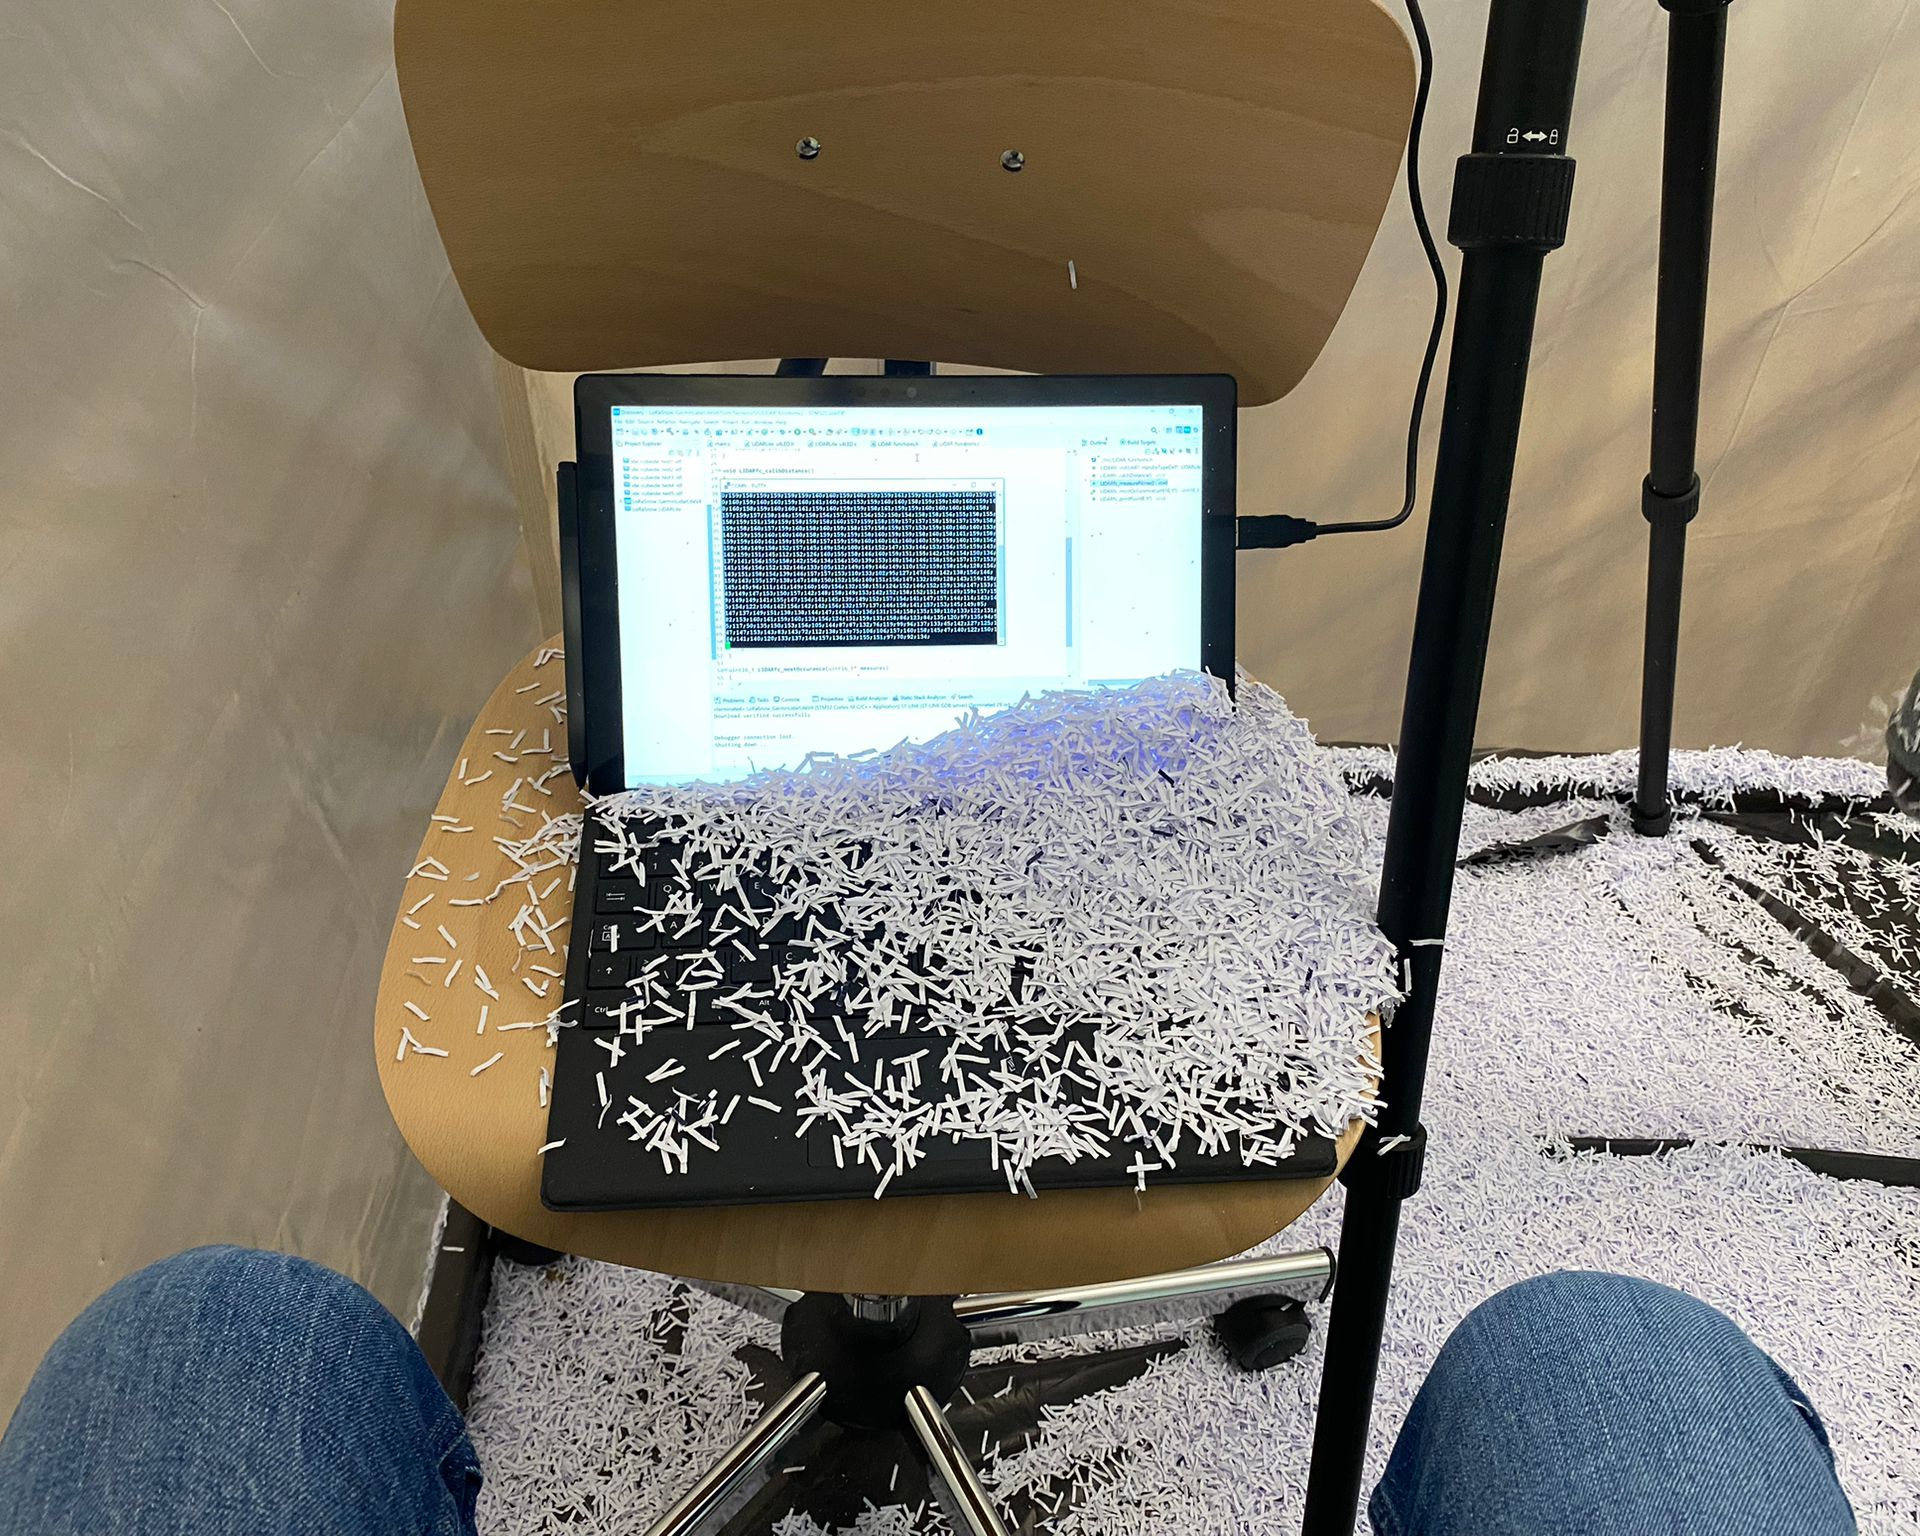
\includegraphics[width=0.35\textwidth]{Images/photos_PGA/canonAction2.PNG}
    \caption{Mise en fonction du canon}
    \label{fig:canonupdate}
\end{figure}

Pour l’assemblage des différentes pièces du canon, comme ces dernières étaient très bien ajustées et 
tenaient entres elles, utiliser des colles fortes spécifiques n’a pas été nécessaire. 
L’utilisation de colle chaude pour garantir un non-détachement et un démontage plus simple a été utilisé. 
Certaines pièces étant interchangeables, elles ne pouvaient pas être collées. Par conséquent, l’utilisation de scotch pour 
garantir aucun déboitement a été privilégié. Cet appareil a surtout été conçu dans un but d'effectuer 
les mesures rapidement et le temps de conception/réalisation était très court. C’est pourquoi la complexité 
des fixations n’a pas été une priorité. L’objectif qui était d’avoir un débit de neige constant a donc 
été atteint. La figure \ref{fig:canonensemble} montre l'assemblage final du canon à confettis.

\begin{figure}[H]
    \centering
    \includegraphics[width=0.4\textwidth]{Images/photos_PGA/canonComplpetv2-removebg-preview.png}
    \caption{Ensemble final du canon à confettis}
    \label{fig:canonensemble}
\end{figure}

\newpage
\section{Boitier}

L’électronique ainsi que les capteurs doivent être protégés, les mesures se passant en milieu non 
favorable (neige, pluie, vents…). La conception du boitier devra assurer une bonne étanchéité des 
composants. Pour cela il faut un boitier sur mesure répondant à beaucoup de critères comme un encombrement 
optimisé, une fixation permettant de mettre le boitier sur plusieurs styles de support et surtout 
une simplicité de conception. Garantir une simplicité de conception dans un encombrement limité est
un défi complexe.\par
La configuration de base du boitier était d’avoir un LiDAR et une caméra qui travaillent ensemble, 
le liDAR permettant d’avoir une mesure de hauteur de neige et la webcam d’avoir une mesure sur le débit 
de neige. Une carte de développement ainsi qu’une carte d'extension spécifique doit être intégré. Une batterie 
permet au système de fonctionner de manière autonome.

\subsection{Vitre}

Le premier défi réside dans le fait d’avoir une partie du boitier transparente tout en gardant ses caractéristiques d'étanchéité, 
le but étant d’incruster une ou plusieurs vitres pour que les capteurs puissent effectuer leurs mesures 
sans être perturbé par des problèmes d’eau ou de poussière. La vitre doit rester remplaçable facilement 
en cas de casse ou d’usure. Un appareil qui est particulièrement étanche et qui permet une vision à 
travers un boitier est la GoPro. Sur les anciens modèles, la vitre est démontable. Le système qui permet 
à cette dernière d’être étanche et composé d’un joint qui vient pincer entre les deux surfaces en contact. 
Le principe étant le même que celui recherché, il a été retenu et adapté.Lla solution est plus 
amplement détaillée à la figure \ref{fig:vitre}, la vitre en bleu vient pincée sur le joint par la plaque du haut. La pression est 
maintenue par les vis ce qui garantit l’étanchéité.

\begin{figure}[H]
    \centering
    \includegraphics[width=0.25\textwidth]{Images/photos_PGA/vitreInv.PNG}
    \includegraphics[width=0.6\textwidth]{Images/photos_PGA/vitreJoint.PNG}
    \caption{Vitre et jointure}
    \label{fig:vitre}
\end{figure}

Dans le cas où ces pièces sont faites en plastique, l’utilisation de vis auto taraudeuse ou d’insert 
filetés seraient utilisés. Les vis auto taraudeuses sont plus simple à mettre en place et tout aussi 
efficace. \\
Dans le cas de pièces métalliques, un simple taraudage suffit. L’utilisation de frein filet est 
envisageable mais étant donné que la pièce sert un joint élastique, il devrait absorber la plupart 
des vibrations.\par 
Pour permettre au capteur de faire des mesures, il faut une zone du boitier transparente. Un verre 
était la solution. Cependant ce n’est pas aussi simple. En effet, le capteur fonctionne dans les infrarouges 
proches (940nm). Tous les verres ne permettent pas le passage de ces rayons. Sur le graphique de la figure \ref{fig:wavelength}, 
la capacité à laisser passer les rayons en fonction de la longueur d’onde est exprimé. Sans étonnement, 
le verre de quartz est le plus adapté.\\
De plus, les verres de quartz et de silice offrent une grande résistance aux hautes températures et 
aux chocs thermiques. Ils ont une grande homogénéité et permettent une excellente transmission de la 
lumière visible, mais aussi des rayonnements ultraviolets et infrarouges proches\footnotemark[1].

%\footnotetext[1]{https://www.researchgate.net/figure/Color-online-Optical-transmittance-spectra-of-quartz-glass-asdeposited-ZnO-and_fig4_274430836}

\begin{figure}[H]
    \centering
    \includegraphics[width=0.7\textwidth]{Images/photos_PGA/wavelength.png}
    \caption{Transmittance de différents matériaux}
    \label{fig:wavelength}
\end{figure}

\subsection{Premier prototype}

\subsubsection{Ouverture}

À la suite de ça, un prototype de boitier a été réalisé pour se rendre compte de l’encombrement, de la 
praticité et du design. Il a été choisi de mettre l'ouverture à l’arrière du boitier, comprenant un
système d’étanchéité démontré sur la figure \ref{fig:vuearriereboitier}. Le maintien de la pression 
sur le joint était fait grâce à quatre vis qui venait directement prendre dans la base du boitier. 
Cette manière de fixer permet de ne pas avoir de trou traversant le boitier. Cette méthode est la 
même que sur celle utilisé dans de la plupart des boitiers étanches.

\begin{figure}[H]
    \centering
    \includegraphics[width=0.4\textwidth]{Images/photos_PGA/Arrièreboitierv3coté.PNG}
    \caption{Ouverture arrière du boitier}
    \label{fig:vuearriereboitier}
\end{figure}

\subsubsection{Encombrement}

Comme le boitier possède un encombrement de 200mm x 100mm x 100mm, il faut une électronique de 
moyenne taille. La figure \ref{fig:encombrementv1} montre l'espace disponible dans le boitier, sans 
les batteries, le capteur et le module d'extension.

\begin{figure}[H]
    \centering
    \includegraphics[width=0.3\textwidth]{Images/photos_PGA/boitierV3.PNG}
    \includegraphics[width=0.4\textwidth]{Images/photos_PGA/boitierV3enc.PNG}
    \caption{Encombrement du boitier, version 1}
    \label{fig:encombrementv1}
\end{figure}

En avançant dans le design du boitier, des difficultés concernant la fixation de l’électronique dans le boiter 
se sont manifesté. L’utilisation d’une casquette devenait aussi complexe, car il faut éviter à tout prix d'avoir
des perçages traversants. La fixation du le bras a été pensée pour se trouver
sous le boitier. Cependant elle aurait aussi pu être prise sur les côtés en englobant la casquette. 
À la suite de tous ces problèmes, le design a été complètement revisité.

\subsection{Version finale du boitier}

Le dernier design est inspiré des caméras de surveillance récente. Ce boitier sera conçu à base de 
polymère, qui permet de limiter les transferts de chaleurs et les coûts.

\subsubsection{Matériaux}

Les deux matériaux les plus souvent retrouvés dans l’industrie pour les boitiers sont l’acrylonitrile 
butadiène styrène (ABS) et le polycarbonate (PC). Le polycarbonate n’apprécie pas d’être exposé trop 
longtemps à un environnement humide. Cela pourrait provoquer de l’hydrolyse et dégrader le boitier. 
L’ABS quant à lui est très résistant. Il est notamment utilisé pour faire des barques de secours.  
L’injection de ce polymère est très répendue. Il est notamment utilisé pour fabriquer les briques \emph{Lego}. 
Ce terpolymère montre une bonne résistance aux chocs jusqu'à -40 °C. Sa température de transition vitreuse se 
situe aux alentours 110 °C, ce qui est largement suffisant dans notre cas. Le problème de l’ABS est qu’il a une mauvaise 
résistance aux rayons UV. L’utilisation d’un revêtement de protection UV sous forme de peinture est envisageable. 
Ce processus permettrait d’augmenter la durée de vie du boitier. Le prix de l’ABS se situe aux alentours 
de 3200 euros la tonne\footnotemark[1].\\
L’aluminium aurait aussi pu être intéressant pour la fabrication de ce boitier. Cependant la fonderie 
s’avère plus complexe et plus couteuse que l’injection plastique. Le prix de la matière aurait quasiment 
triplé. Les caractéristiques du polymère étant parfaitement suffisantes, l’intérêt d’utiliser de l’aluminium 
n’était donc pas nécessaires.

\footnotetext[1]{https://www.polyvia.fr/fr/prix-du-plastique-les-previsions-pour-2022}

\subsubsection{Ouverture}

L’ouverture se fait par en haut à l’aide d’un couvercle amovible. Le système d’étanchéité est le 
même que les précédentes versions. Le maintien en pression sur le joint est effectué grâce à 
une fixation dites grenouillère, comme le montre la figure \ref{fig:ouverturev2}. La grenouillère 
dispense l’utilisation d’outils et permet un gain de temps lors de l’ouverture et la fermeture. 
Cette dernière possède une serrure intégrée pour dissuader de possibles vols.

\begin{figure}[H]
    \centering
    \includegraphics[width=0.4\textwidth]{Images/photos_PGA/Boitierv41.PNG}
    \includegraphics[width=0.35\textwidth]{Images/photos_PGA/grenouillère.PNG}
    \caption{Ouverture du boitier, version 2 (à gauche), grenouillère pour la fermeture (à droite)}
    \label{fig:ouverturev2}
\end{figure}

\subsubsection{Pivot du couvercle}

L’une des grandes forces de ce systèmes est son ouverture simplifiée. En effet, le couvercle est fixé 
comme une trappe. Cette spécificité permet d’avoir un bien meilleur accès à l’intérieur du système. 
Cette particularité permet pouvoir manipuler aisément les éléments qui se situent à l’intérieur. Le 
pivot est assuré par un axe (tube) fileté à ses deux extrémités. Deux vis viennent maintenir de chaque 
côté l’axe afin qu’il ne puisse pas sortir de son logement. Le système d'ouverture est représenté à la 
figure \ref{fig:pivot}.

\begin{figure}[H]
    \centering
    \includegraphics[width=0.25\textwidth]{Images/photos_PGA/pivotcoupe.PNG}
    \includegraphics[width=0.6\textwidth]{Images/photos_PGA/pivotnormal.PNG}
    \caption{Mécanisme du pivot}
    \label{fig:pivot}
\end{figure}

\subsubsection{Fixation de la casquette}

La casquette qui se situe sur le couvercle est facilement démontable pour mettre un autre modèle ou 
la changer en cas de dégradation Elle est fixée par quatre vis imbus qui viennent se loger dans des inserts 
situés sur le dessus du couvercle. Les fixations de la casquette sont posées sur le couvercle, cette 
configuration permet de soulager les efforts sur les supports, comme le montre la figure \ref{fig:casquette}.

\begin{figure}[H]
    \centering
    \includegraphics[width=0.4\textwidth]{Images/photos_PGA/fixcasquette.PNG}
    \includegraphics[width=0.4\textwidth]{Images/photos_PGA/inserts.jpg}
    \caption{Mécanisme du pivot}
    \label{fig:casquette}
\end{figure}

\subsubsection{Fixation du module}

En ce qui concerne la partie intérieure, quatre supports sont intégrés dans le fond du boitier. Ces derniers 
sont dimensionnés pour accueillir des inserts plastiques. Toute la partie électronique pourra par la 
suite venir se fixer sur le dessus. La figure \ref{fig:fixbase} montre ces fixations.

\begin{figure}[H]
    \centering
    \includegraphics[width=0.35\textwidth]{Images/photos_PGA/fixationbaseModule.PNG}
    \caption{Fixation du module}
    \label{fig:fixbase}
\end{figure}

\subsubsection{Fixations des supports}

La fixation du bras sera assurée par quatre écrous carrés situé sous le boitier, comme le montre la figure 
\ref{fig:supportfix}. Cette solution permet de 
ne pas à avoir à faire de trous dans le boitier pour maintenir une bonne étanchéité. Ces écrous sont 
guidés dans une gorge afin d’être maintenus pendant le serrage. Le même principe est utilisé pour 
fixer des éléments dans les armoires d'automation.

\begin{figure}[H]
    \centering
    \includegraphics[width=0.4\textwidth]{Images/photos_PGA/fixdessous2.PNG}
    \includegraphics[width=0.4\textwidth]{Images/photos_PGA/écroucarré.PNG}
    \caption{Support de fixation du boitier}
    \label{fig:supportfix}
\end{figure}

\subsection{Module électronique}

Cette partie est consacrée au développement d’un module compact et simple composé de toute l'électronique, 
comme montré sur la figure \ref{fig:elmodule}.
Ce module est fixé dans le boitier grâce aux quatre plots de fixations situés dans le fond 
du boitier. L’interêt de designer une construction mécanique est de pouvoir soutenir tous les composants 
pour les empêcher de se déplacer à leur guise. La simplicitée recherchée dans sa conception permet
aux opérateurs de gagner du temps.

\begin{figure}[H]
    \centering
    \includegraphics[width=0.5\textwidth]{Images/photos_PGA/ModuleElec2-removebg-preview.png}
    \caption{Module électronique}
    \label{fig:elmodule}
\end{figure}

\subsubsection{Base du support des batteries}

La pièce de base est prévue pour accueillir 6 batteries 18650, que l'on retrouve à la figure \ref{fig:supportbatteries}.
Un espace légèrement plus grand est 
prévu. L’appellation 18650 signifie que l’élément rechargeable fait un diamètre de 18mm et une longueur 
de 65mm. Des petites fentes ont aussi été pensées pour faciliter un câblage série/parallèle entre les 
éléments. Cette pièce est la fondation du module électronique, elle sera naturellement fixée dans le 
boitier grâce aux 4 trous de fixations.

\begin{figure}[H]
    \centering
    \includegraphics[width=0.4\textwidth]{Images/photos_PGA/moduleFondbat.PNG}
    \includegraphics[width=0.4\textwidth]{Images/photos_PGA/bateriebl.PNG}
    \caption{Support à batteries}
    \label{fig:supportbatteries}
\end{figure}

\subsubsection{Plaque de fixation et PCB}

Au-dessus de la pièce supportant les batteries, une plaque est fixée. Cette dernière est très importante 
dans l’ensemble. Elle permet grâce aux trois fixations situées aux extrémités de venir bloquer les batteries 
pour éviter qu'elles ne bougent. Ces trois trous sont prévus pour venir fixer la plaque 
sur le module du bas. Les quatre autres servent à fixer la partie PCB. Quatre vis à tête fraisée seront 
insérées dans les trous fraisés afin de venir fixer des entretoises en plastiques. Sur ces dernières, 
les circuits imprimés pourront être fixé à l’aide de visses en plastiques. Ces composants 
plastique permettent d’éviter tout risque de court-circuit. La figure \ref{fig:fixelectronique} montre la plaque
de fixation et le module électronique monté.

\begin{figure}[H]
    \centering
    \includegraphics[width=0.4\textwidth]{Images/photos_PGA/plaquesmodule.PNG}
    \includegraphics[width=0.4\textwidth]{Images/photos_PGA/PCB.PNG}
    \caption{Plaque de fixation pour la partie électronique}
    \label{fig:fixelectronique}
\end{figure}

\subsubsection{Support du LiDAR}

Le capteur LiDAR ne possède pas de trou de fixation, seul deux fentes sont disponibles pour venir 
cliper un support sur ce dernier. Le fabricant préconise de le fixer avec des attaches plastiques ou du scotch 
double face. Ces solutions sont plutôt prévues à des fins de bricolage. Des essais de supports à base 
de clips ont été réalisé mais l’ajustement de ces derniers était problématique. C’est pour ça que la 
solution de pincer le capteur à l’aide de vis sans tête est parvenue comme la plus sûre et la plus simple. 
Le support qui permet de fixer le LiDAR dans la bonne position vient directement se fixer dans les 
trous de fixations du support à batteries. La figure \ref{fig:supportlidar} montre sous différents angles 
le support.

\begin{figure}[H]
    \centering
    \includegraphics[width=0.3\textwidth]{Images/photos_PGA/lidar dans support.png}
    \includegraphics[width=0.3\textwidth]{Images/photos_PGA/supportLidar2.PNG}
    \includegraphics[width=0.3\textwidth]{Images/photos_PGA/supportlidar.PNG}
    \caption{Support pour le LiDAR}
    \label{fig:supportlidar}
\end{figure}

\subsection{Bras de fixation}

La partie fixation permet d’assurer un positionnement juste et précis de l’ensemble du boitier. Cette 
dernière doit pouvoir se faire sur quasiment toutes les surfaces à dispositions comme les murs ou les 
lampadaires.

\subsubsection{Support du boitier}

Le support du boitier est une partie rigide en aluminium qui vient se visser sous le boitier à l’aide 
quatre vis. Cette pièce est en deux partie. La première partie est une plaque carrée ayant les trous de 
perçage correspondant au boitier. La deuxième est une autre plaque percée soudée perpendiculairement.
Ce perçage permettra de jongler entre les systèmes de fixation désiré. Grace à cette liaison par boulon, 
l’inclinaison du boitier pourra être réglée.\\
En ce qui concerne le réglage précis de l’angle, un petit cadran autocollant pourrait être rajouté 
sur le support et une ligne autocollante sur le support du boitier. Elle permettra de lire la valeur 
de l’inclinaison du boitier. Cette petite subtilité permettra de faciliter le montage du boitier et 
de pouvoir contrôler si la position est bonne sur le long terme.\\
La figure \ref{fig:angle} montre la fixation au boitier ainsi que le réglage d'angle.

\begin{figure}[H]
    \centering
    \includegraphics[width=0.5\textwidth]{Images/photos_PGA/fixdessous2.PNG}
    \includegraphics[width=0.32\textwidth]{Images/photos_PGA/mesure d'angle.PNG}
    \caption{Système de réglage de l'élévation}
    \label{fig:angle}
\end{figure}

\subsubsection{Support mural et tubulaire}

L’objectif voulu est de pouvoir fixer le boitier sur des lampadaires ou des poteaux. Un système de 
collier de serrage a donc été conçu pour répondre à cette problématique. Les deux arcs de cercle collé 
entre eux forment un ovale avec une aire plus petite que celle du poteau de fixation. En venant 
serrer les vis, une force de serrage agira naturellement sur le poteau et le boitier sera bien fixé. 
Afin de régler la rotation azimutale, c’est-à-dire autours de l’axe du lampadaire, il suffit de placer 
le boitier dans la position voulue. Une fois cette position atteinte, il faut bloquer l’ensemble boulonné. 
Ce dispositif permet deux degrés de liberté, l’azimut et l’élévation. La figure \ref{fig:supfix} montre 
les deux supports possibles de fixation.

\begin{figure}[H]
    \centering
    \includegraphics[width=0.4\textwidth]{Images/photos_PGA/collierSupport2.PNG}
    \includegraphics[width=0.3\textwidth]{Images/photos_PGA/supportmural2.PNG}
    \caption{Support de fixation tubulaire et mural}
    \label{fig:supfix}
\end{figure}

Un autre dispositif pour une fixation murale a aussi été pensé. Malheureusement dans cette configuration 
la rotation azimutale ne peut pas être réglée. Le seul degré de liberté est l’élévation. Les trous en 
bleus ont été pensés pour passer un éventuel collier de serrage pour un fixation spécial ou un montage 
provisoire.

\subsection{LoRaSnow Testbox}

Pour savoir si les simulations effectuées correspondaient avec la réalité, il a fallu tester le capteur 
en condition réelle. Cependant les chutes de neiges sont difficilement prévisibles. Le boitier final était 
encore au stade de conception, il a fallu confectionner un élément temporaire pour protéger les composants 
durant les essais. Le LiDAR a été fixé sous le boitier à l'aide de la fixation avec les clips. Ce type de fixation 
n’étant pas convainquant, une attache plastique a été rajouté pour augmenter la force de pincement des clips. 
Une autre fixation permettait de visser le boitier sur un trépied. La figure \ref{fig:testbox} montre le boitier 
temporaire ainsi que sa fixation.

\begin{figure}[H]
    \centering
    \includegraphics[width=0.45\textwidth]{Images/photos_PGA/TestBox-removebg-preview.png}
    \includegraphics[width=0.35\textwidth]{Images/photos_PGA/testboxinside.jpg}
    \caption{LoRaSnow Testbox, intérieur et extérieur}
    \label{fig:testbox}
\end{figure}

%% HEEEEEEEEEEEEEEEEEEEEEEEEEEHHHHHH STOOOOOOOOOOOOOOOOOPPPPPPPPPPPPPPP %%

\section{Synthèse des résultats}

Grace à un banc de test comprenant une cage d’essai et un canon à confettis. Plusieurs séries de mesures 
concluantes ont pu être réalisées. Le débit de neige produit par le canon étant réglable, il augmente les 
possibilités de mesures. La cage permit de contenir les nuages de confettis sans dégrader les conditions 
de travails des autres usagers de la salle.\\
Différents designs de boitier ont été imaginés avant d’arriver à la solution finale. L’étanchéité fut la 
partie plus problématique lors de la conception. L’utilisation de joint torique pincé permit de résoudre 
ces problèmes. L’ABS étant une matière très simple à injecter, la fabrication des pièces du boitier serait 
corolaire. Le support du boitier permet de régler à la fois l’élévation et l’azimut du boitier. La partie 
amovible supérieure permet un très bon accès à la partie du module électronique. Elle se verrouille facilement 
grâce à une fermeture par grenouillère. L’ouverture est verrouillée grâce à la serrure incrustée dans la 
fixation.\\
Le module électronique se fixe simplement dans le boitier à l’aide de 4 vis. Une structure mécanique permet 
de maintenir les batteries en place. Au-dessus des batteries, une plaque permet la fixation du capteur Lidar 
et des PCB. Suffisamment d’espace est prévu autour du module afin de pouvoir disposer aisément le câblage. 
La simplicité du module permet une manipulation rapide et simple des différents éléments.